% ============================================================================
%  ADVANCED COMPUTER ARCHITECTURE LECTURE NOTES
%  UNIT 1: Theory of Parallelism & Parallel Computer Models
% ============================================================================

\documentclass[11pt,a4paper]{article}

% ── Fonts ───────────────────────────────────────────────────────────────────
% \usepackage{mathpazo}
\usepackage[T1]{fontenc}
% \linespread{1.05}
\usepackage{noto}

% ── Typography ──────────────────────────────────────────────────────────────
% \usepackage[protrusion=true, expansion=true]{microtype}
% \usepackage{setspace}
% \onehalfspacing

% ── Page Layout ─────────────────────────────────────────────────────────────
\usepackage[
  a4paper,
  left=1in,
  right=1in,
  top=1.15in,
  bottom=1.15in,
  headheight=22pt
]{geometry}

% ── Colors ──────────────────────────────────────────────────────────────────
\usepackage[dvipsnames,svgnames,table]{xcolor}

\definecolor{TheoremBlue}{RGB}{0,82,155}
\definecolor{DefinitionGreen}{RGB}{0,112,74}
\definecolor{ExampleOrange}{RGB}{184,84,0}
\definecolor{RemarkPurple}{RGB}{108,52,131}
\definecolor{ProofBorder}{RGB}{120,120,160}
\definecolor{NoteRed}{RGB}{179,0,0}
\definecolor{ChapterBlue}{RGB}{20,60,120}

% ── Math Packages ───────────────────────────────────────────────────────────
\usepackage{amsmath,amssymb,amsthm,mathtools}
\usepackage{mathrsfs}
\usepackage{bbm}

% ── Theorem Environments (tcolorbox) ────────────────────────────────────────
\usepackage[most]{tcolorbox}
\tcbuselibrary{theorems, skins, breakable}

\newtcbtheorem[number within=section]{theorem}{Theorem}{%
  enhanced,
  colback=TheoremBlue!4,
  colframe=TheoremBlue!80!black,
  coltitle=white,
  fonttitle=\bfseries,
  sharp corners,
  boxrule=0.8pt,
  top=6pt, bottom=6pt, left=8pt, right=8pt,
  separator sign none,
  description delimiters parenthesis,
  breakable
}{thm}

\newtcbtheorem[number within=section]{definition}{Definition}{%
  enhanced,
  colback=DefinitionGreen!4,
  colframe=DefinitionGreen!70!black,
  coltitle=white,
  fonttitle=\bfseries,
  rounded corners,
  boxrule=0.8pt,
  top=6pt, bottom=6pt, left=8pt, right=8pt,
  separator sign none,
  description delimiters parenthesis,
  breakable
}{def}

\newtcbtheorem[number within=section]{example}{Example}{%
  enhanced,
  colback=ExampleOrange!4,
  colframe=ExampleOrange!60!black,
  fonttitle=\bfseries,
  rounded corners,
  boxrule=0.6pt,
  borderline west={3pt}{0pt}{ExampleOrange!80},
  top=5pt, bottom=5pt, left=10pt, right=8pt,
  separator sign none,
  breakable
}{ex}

\newtcolorbox{remark}[1][]{%
  enhanced,
  colback=RemarkPurple!3,
  colframe=RemarkPurple!3,
  borderline west={2.5pt}{0pt}{RemarkPurple!70},
  sharp corners,
  boxrule=0pt,
  top=5pt, bottom=5pt, left=8pt, right=8pt,
  fontupper=\small,
  before upper={\textbf{\color{RemarkPurple}Remark.}\quad},
  breakable,
  #1
}

\newtcolorbox{notebox}[1][]{%
  enhanced,
  colback=NoteRed!3,
  colframe=NoteRed!3,
  borderline west={2.5pt}{0pt}{NoteRed!70},
  sharp corners,
  boxrule=0pt,
  top=5pt, bottom=5pt, left=8pt, right=8pt,
  before upper={\textbf{\color{NoteRed}Note.}\quad},
  breakable,
  #1
}

% ── TikZ Diagrams ───────────────────────────────────────────────────────────
\usepackage{tikz}
\usetikzlibrary{positioning, arrows.meta, shapes.geometric, calc, fit, backgrounds}

\tikzset{
  box/.style={draw, rectangle, rounded corners, fill=blue!10, minimum width=2.2cm, minimum height=1cm, align=center, font=\small},
  mem/.style={draw, rectangle, fill=green!10, minimum width=4cm, minimum height=1cm, align=center, font=\small},
  net/.style={draw, double, fill=orange!10, minimum width=6cm, minimum height=0.8cm, align=center, font=\small\bfseries},
  node/.style={circle, draw=blue!80, fill=blue!15, minimum size=8mm, font=\small\bfseries}
}

% ── Lists ───────────────────────────────────────────────────────────────────
\usepackage[shortlabels]{enumitem}
\setlist[enumerate]{topsep=4pt, itemsep=2pt, parsep=2pt}
\setlist[itemize]{topsep=4pt, itemsep=2pt, parsep=2pt}
\setlist[enumerate,1]{label=\arabic*.}

% ── Tables ──────────────────────────────────────────────────────────────────
\usepackage{booktabs}
\usepackage{array}
\usepackage{tabularx}

% ── Headers and Footers ────────────────────────────────────────────────────
\usepackage{fancyhdr}
\pagestyle{fancy}
\fancyhf{}
\fancyhead[L]{\small\textcolor{ChapterBlue}{\nouppercase{\leftmark}}}
\fancyhead[R]{\small\textcolor{ChapterBlue}{\thepage}}
\renewcommand{\headrulewidth}{0.4pt}
\renewcommand{\headrule}{\hbox to\headwidth{%
  \color{ChapterBlue}\leaders\hrule height \headrulewidth\hfill}}
\fancypagestyle{plain}{%
  \fancyhf{}
  \fancyfoot[C]{\small\textcolor{ChapterBlue}{\thepage}}
  \renewcommand{\headrulewidth}{0pt}
}

% ── Section Styling ─────────────────────────────────────────────────────────
\usepackage{titlesec}
\titleformat{\section}
  {\Large\bfseries\color{ChapterBlue}}
  {\thesection}{0.8em}{}

\titleformat{\subsection}
  {\large\bfseries\color{DefinitionGreen!80!black}}
  {\thesubsection}{0.7em}{}

\titleformat{\subsubsection}
  {\normalsize\bfseries\color{ExampleOrange!80!black}}
  {\thesubsubsection}{0.6em}{}

% ── Hyperlinks ──────────────────────────────────────────────────────────────
\usepackage{hyperref}
\hypersetup{
  colorlinks=true,
  linkcolor=TheoremBlue!80!black,
  citecolor=DefinitionGreen,
  urlcolor=TheoremBlue,
  bookmarksnumbered=true,
  pdfstartview=FitH
}
\usepackage[nameinlink,capitalize]{cleveref}

% ============================================================================
%  DOCUMENT BEGINS
% ============================================================================
\begin{document}

\begin{titlepage}
\centering
\vspace*{1.5cm}

{\color{ChapterBlue}\rule{\textwidth}{1.5pt}}
\vspace{0.6cm}
{\fontsize{26}{32}\selectfont\bfseries\color{ChapterBlue} Advanced Computer Architecture}
\vspace{0.4cm}
{\Large\color{gray} Academic Student Notes}
\vspace{0.4cm}
{\color{ChapterBlue}\rule{\textwidth}{1.5pt}}

\vspace{1cm}
{\large\textbf{UNIT - I: Theory of Parallelism \& Parallel Computer Models}}

\vspace{1.5cm}

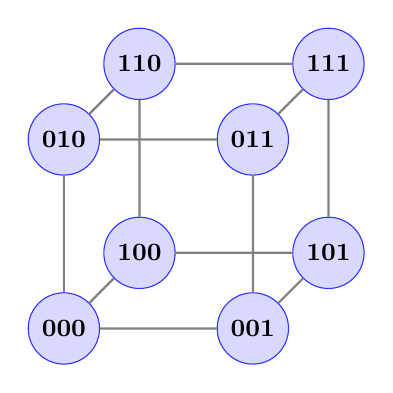
\begin{tikzpicture}[scale=1.2]
  % Draw a simple Hypercube (3D) to look professional
  \node[node] (0) at (0,0) {000};
  \node[node] (1) at (2,0) {001};
  \node[node] (2) at (2,2) {011};
  \node[node] (3) at (0,2) {010};
  
  \node[node] (4) at (0.8,0.8) {100};
  \node[node] (5) at (2.8,0.8) {101};
  \node[node] (6) at (2.8,2.8) {111};
  \node[node] (7) at (0.8,2.8) {110};
  
  % Lower/Front face edges
  \draw[thick, gray] (0) -- (1) -- (2) -- (3) -- (0);
  % Upper/Back face edges
  \draw[thick, gray] (4) -- (5) -- (6) -- (7) -- (4);
  % Interconnecting edges
  \draw[thick, gray] (0) -- (4);
  \draw[thick, gray] (1) -- (5);
  \draw[thick, gray] (2) -- (6);
  \draw[thick, gray] (3) -- (7);
\end{tikzpicture}

\vspace{1.5cm}
{\large\textit{Department of Computer Science and Engineering}} \\
\vspace{0.2cm}
{\large\textbf{Marri Laxman Reddy Institute of Technology and Management}} \\
\vspace{0.1cm}
{\small (UGC Autonomous, R25 Regulation)}

\vfill
{\normalsize Compiled: \today}
\end{titlepage}

\tableofcontents
\newpage

% ============================================================================
\section{Theory of Parallelism \& The State of Computing}
% ============================================================================

Imagine you are hosting a large dinner party. If you are the only cook in the kitchen, preparing the soup, the salad, the main course, and the dessert one by one takes a very long time. This is how \textbf{sequential computing} works—one instruction after another. 

\textbf{Parallel processing} is like hiring four chefs who work in the kitchen at the same time: one chops vegetables, one stirs the soup, one bakes the main dish, and one plates the dessert. By dividing the work, dinner is ready in a fraction of the time. 

In computer science, we are forced to build parallel computers because single-processor chips have hit a physical limit—they get too hot and consume too much power if we try to make them run any faster sequentially.

\subsection{Architectural Development Tracks}
To understand how computers got to where they are today, we can trace three historical paths of evolution:

\begin{enumerate}
    \item \textbf{The Processor Track (Instruction-Level Parallelism - ILP)}:
    How does a single core execute tasks faster?
    \begin{gather*}
        \text{SISD (Single Chef)} \longrightarrow \text{Pipelining (Assembly Line)} \\
        \longrightarrow \text{Superscalar (Two Hands)} \longrightarrow \text{VLIW (Pre-packaged tasks)} \\
        \longrightarrow \text{SMT (Multitask while waiting)} \longrightarrow \text{Multi-Core (Multiple Kitchens)}
    \end{gather*}
    Instead of just running one command at a time, modern processors use assembly lines (pipelining) where one instruction is fetched while another is decoded and a third is executed.

    \item \textbf{The Memory Track (Memory Wall \& Caching)}:
    Imagine a super-fast chef who chops ingredients at lightning speed, but has to walk to a warehouse across town (the main memory) to get every single onion or potato. The chef spends $99\%$ of their time walking, not chopping. This delay is called the \textbf{Memory Wall}.
    To solve this, we place small, fast baskets of ingredients directly next to the cutting board (L1, L2, L3 caches). The chef checks the baskets first; only if something is missing do they make the long trip to the warehouse.

    \item \textbf{The Control Track (How instructions are triggered)}:
    \begin{itemize}
        \item \textbf{Control-Flow}: Traditional programming. A program counter points to step 1, then step 2, then step 3.
        \item \textbf{Data-Flow}: No program counter. An instruction executes the exact millisecond its inputs become available. (Like a factory station that glues a label on a box as soon as both a box and a label slide down the belt).
        \item \textbf{Reduction (Demand-Flow)}: Work is triggered only when someone asks for a result. (Like a restaurant where cooking only begins when a customer orders a specific meal).
    \end{itemize}
\end{enumerate}

\subsection{Theoretical Models: PRAM and VLSI}

To study parallel algorithms without getting bogged down by specific hardware models, scientists use simplified mathematical models:

\begin{definition}{PRAM (Parallel Random Access Machine)}{pram}
Imagine a classroom with $p$ students (processors) who share a single large blackboard (shared memory). Any student can read from or write to any part of the blackboard in exactly $1$ unit of time. 
\end{definition}

Since multiple students might try to look at or write on the same section of the board at the same time, we have different rules for access:
\begin{itemize}
    \item \textbf{EREW} (Exclusive Read, Exclusive Write): Only one student can look at or write to a specific board section at a time. No sharing allowed during that step.
    \item \textbf{CREW} (Concurrent Read, Exclusive Write): Multiple students can read from the same section at the same time, but only one student is allowed to write to it at a time.
    \item \textbf{CRCW} (Concurrent Read, Concurrent Write): Multiple students can read and write simultaneously. If they write to the exact same spot, we need a tie-breaker rule:
    \begin{itemize}
        \item \textit{Common}: All students writing to that spot must write the exact same word.
        \item \textit{Arbitrary}: One random student's write succeeds, others are discarded.
        \item \textit{Priority}: The student with the lowest roll number (highest priority) gets to write.
    \end{itemize}
\end{itemize}

\begin{definition}{VLSI Complexity Model}{vlsi}
Unlike mathematical models, physical microchips have space constraints. The \textbf{VLSI model} evaluates algorithms based on:
\begin{itemize}
    \item $A$: The silicon area of the chip (how much physical space and wiring it needs).
    \item $T$: The execution time of the algorithm.
\end{itemize}
There is a trade-off represented by $AT^2 = \Omega(f(n))$. If you want an algorithm to execute twice as fast ($T/2$), you will need a chip with four times the wiring area ($4A$) to route all the parallel signals.
\end{definition}

% ============================================================================
\section{Parallel Computer Models}
% ============================================================================

We categorize parallel computers based on how they organize their processors and memory.

\subsection{Multiprocessors (Shared-Memory Systems)}
In a multiprocessor system, all processors share a single, giant pool of memory. If Processor 1 writes a value to memory address \texttt{100}, Processor 2 can read it instantly. 

\textit{Analogy}: Imagine a group of friends sitting around a single table, building one giant jigsaw puzzle together. Everyone can see and touch the entire puzzle.

\begin{center}
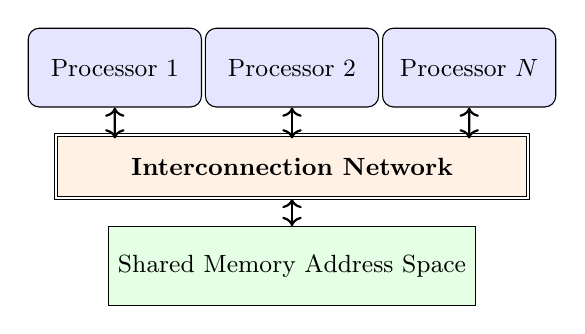
\begin{tikzpicture}[scale=0.9]
  \node[box] (P1) at (-2.5, 1.8) {Processor 1};
  \node[box] (P2) at (0, 1.8) {Processor 2};
  \node[box] (Pn) at (2.5, 1.8) {Processor $N$};
  
  \node[net] (ICN) at (0, 0.4) {Interconnection Network};
  
  \node[mem] (Mem) at (0, -1) {Shared Memory Address Space};
  
  \draw[thick, <->] (P1) -- (-2.5, 0.8);
  \draw[thick, <->] (P2) -- (0, 0.8);
  \draw[thick, <->] (Pn) -- (2.5, 0.8);
  \draw[thick, <->] (ICN) -- (Mem);
\end{tikzpicture}
\end{center}

We divide shared-memory systems based on memory access speeds:
\begin{enumerate}
    \item \textbf{UMA} (Uniform Memory Access): Every processor takes the exact same amount of time to access any memory location. (Like a circular dining table where all food platters are equally close to everyone).
    \item \textbf{NUMA} (Non-Uniform Memory Access): Memory is split into local blocks near each processor. Accessing your own local memory is super fast, but accessing another processor's local memory across the chip takes longer. (Like a long banquet table where the salad is right in front of you, but you have to ask someone to pass the dessert from the far end).
    \item \textbf{COMA} (Cache-Only Memory Access): There is no static main memory location. The memory behaves like a set of floating caches. Data dynamically migrates to whichever processor is currently using it. (Like sliding the pizza box to whoever is currently hungry).
\end{enumerate}

\subsection{Multicomputers (Distributed-Memory Systems)}
In a multicomputer, each processor has its own private memory. Processor 1 cannot touch or see Processor 2's memory. To share information, they must explicitly send messages to each other over a network.

\textit{Analogy}: Imagine a group of friends working on their own individual sections of a project, each in their own separate house. To coordinate, they must send each other emails or text messages.

\begin{center}
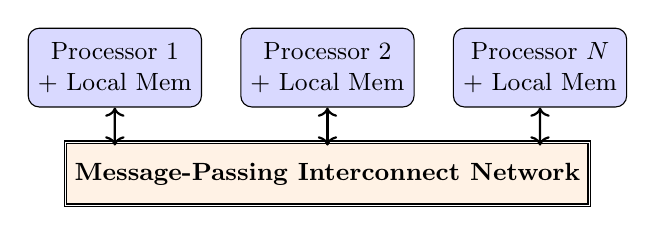
\begin{tikzpicture}[scale=0.9]
  \node[box, fill=blue!15] (N1) at (-3, 1.5) {Processor 1 \\ + Local Mem};
  \node[box, fill=blue!15] (N2) at (0, 1.5) {Processor 2 \\ + Local Mem};
  \node[box, fill=blue!15] (Nn) at (3, 1.5) {Processor $N$ \\ + Local Mem};
  
  \node[net] (ICN) at (0, 0) {Message-Passing Interconnect Network};
  
  \draw[thick, <->] (N1) -- (-3, 0.4);
  \draw[thick, <->] (N2) -- (0, 0.4);
  \draw[thick, <->] (Nn) -- (3, 0.4);
\end{tikzpicture}
\end{center}

\begin{notebox}
Multicomputers are also called \textbf{NORMA (No-Remote Memory Access)} systems. They scale up to thousands of computers easily because there is no single central memory bottleneck that everyone is fighting over.
\end{notebox}

\subsection{Comparison Matrix}
Here is a side-by-side comparison of the two systems:

\begin{table}[h]
\centering
\caption{Multiprocessors vs. Multicomputers}
\begin{tabularx}{\textwidth}{@{}lXX@{}}
\toprule
\textbf{Feature} & \textbf{Multiprocessors (Shared Memory)} & \textbf{Multicomputers (Distributed Memory)} \\ \midrule
Memory Address Space & Single global pool of memory. & Separate private memory for each node. \\
How they talk & Read and write shared variables. & Explicitly send/receive network messages. \\
Scalability Limits & Hard to scale (too many processors choke the memory bus). & Highly scalable (just add more independent computers). \\
Cache Coherence & Needs complex hardware to ensure no one reads stale data. & Not applicable (no shared variables exist). \\
Programming difficulty & Easier to write, but debugging race conditions is a nightmare. & Harder to write (you must partition the data yourself). \\ \bottomrule
\end{tabularx}
\end{table}

\subsection{Vector and SIMD Computers}
\begin{itemize}
    \item \textbf{SIMD (Single Instruction, Multiple Data)}: Imagine a gym class where the instructor shouts: \textit{``Do a jumping jack!''}. Everyone executes the exact same instruction at the exact same time, but they do it using their own bodies (local data). This is how modern GPUs process millions of pixels at once.
    \item \textbf{Multivector Computers}: Specialized machines that execute operations on large arrays (vectors) of numbers. Instead of doing one addition at a time, they feed vectors through deep arithmetic pipelines like an assembly line.
\end{itemize}

% ============================================================================
\section{Program and Network Properties}
% ============================================================================

\subsection{Conditions of Parallelism}
Before running two tasks at the same time, we must ensure they do not interfere with each other. This is formalised by \textbf{Bernstein's Conditions}.

Let $S_1$ and $S_2$ be two statements. Let $I$ be the variables they read (Inputs), and $O$ be the variables they write to (Outputs).

\begin{theorem}{Bernstein's Conditions}{bernsteins}
Two statements $S_1$ and $S_2$ can run safely in parallel if and only if they satisfy three simple rules:
\begin{align}
    I_1 \cap O_2 &= \emptyset \quad (\text{Rule 1: S1 must not read what S2 is writing}) \\
    O_1 \cap I_2 &= \emptyset \quad (\text{Rule 2: S2 must not read what S1 is writing}) \\
    O_1 \cap O_2 &= \emptyset \quad (\text{Rule 3: They must not write to the same location})
\end{align}
\end{theorem}

\begin{example}{Applying Bernstein's Conditions}{bernstein_ex}
Let's analyze three instructions to see if we can run them at the same time:
\begin{itemize}
    \item $S_1$: $A = X + Y$ \hfill (Reads $X, Y$; Writes $A$)
    \item $S_2$: $B = A \times 2$ \hfill (Reads $A$; Writes $B$)
    \item $S_3$: $X = C - D$ \hfill (Reads $C, D$; Writes $X$)
\end{itemize}

\textit{Can $S_1$ and $S_2$ run together?} 
No. $S_1$ writes $A$, and $S_2$ needs to read $A$ to do its calculation. If they run at the same time, $S_2$ might read the old value of $A$ before $S_1$ updates it. This is a \textbf{Flow Dependency}.

\textit{Can $S_1$ and $S_3$ run together?} 
No. $S_1$ needs to read $X$, and $S_3$ is updating $X$. If they run at the same time, $S_1$ might read the new value of $X$ instead of the old one. This is an \textbf{Anti-dependency}.
\end{example}

\subsection{Types of Program Dependencies}
What stops us from running code in parallel? Five main obstacles:
\begin{itemize}
    \item \textbf{Flow (Data) Dependency (Read-After-Write)}: You cannot eat ($S_2$) until I finish cooking ($S_1$).
    \item \textbf{Anti-dependency (Write-After-Read)}: I want to overwrite a page ($S_2$), but I must wait until you finish reading it ($S_1$) so I don't destroy your data.
    \item \textbf{Output Dependency (Write-After-Write)}: We both try to write our names on the same line. If we do it at the same time, the text gets scribbled over.
    \item \textbf{Control Dependency}: You cannot decide to open your umbrella ($S_2$) until you evaluate whether it is raining ($S_1$).
    \item \textbf{Resource Dependency}: We both want to cook, but there is only one frying pan in the kitchen. One of us has to wait.
\end{itemize}

\subsection{Program Partitioning, Grain Size \& Scheduling}
How do we split a large task among multiple processors?
\begin{itemize}
    \item \textbf{Grain Size}: This is the amount of work a processor does before it needs to communicate or synchronize with others.
    \begin{itemize}
        \item \textit{Fine-grain (Tiny tasks)}: Split the work into single sentences. Excellent parallelism, but processors spend all their time talking to each other rather than doing actual work (high communication overhead).
        \item \textit{Coarse-grain (Large tasks)}: Split the work into whole chapters. Low communication overhead, but some processors might finish early and sit idle while waiting for the others (unbalanced load).
    \end{itemize}
    \item \textbf{Scheduling}: The art of assigning these split tasks to the available cores. Good scheduling keeps all cores busy and minimizes the overhead of managing them.
\end{itemize}

\subsection{Program Flow Mechanisms}
How does a computer decide which instruction to run next?
\begin{enumerate}
    \item \textbf{Control-Driven}: Sequential execution guided by a program counter (the classic von Neumann model).
    \item \textbf{Data-Driven (Dataflow)}: Instructions wait passively until all their operands are ready, and then they execute immediately. No program counter exists.
    \item \textbf{Demand-Driven (Reduction)}: The program starts from the desired result and works backward, only triggering calculations that are absolutely necessary to find that result.
\end{enumerate}

% ============================================================================
\section{System Interconnect Architectures}
% ============================================================================

To let processors and memory modules talk to each other, we connect them using networks.

\subsection{Static Interconnection Networks}
In static networks, the connections are permanent copper wires or optical links.
\begin{itemize}
    \item \textbf{Network Diameter}: The maximum number of hops a message must take to travel between the two farthest nodes in the network. (Like the worst-case travel distance in a subway system).
    \item \textbf{Linear Array}: Nodes connected in a straight line. Network diameter is $N-1$ (very slow for large networks).
    \item \textbf{Ring}: A linear array where the ends are joined to make a circle. The diameter is cut in half to $\lfloor N/2 \rfloor$.
    \item \textbf{Mesh}: Nodes arranged in a grid. Diameter for an $r \times c$ grid is $(r-1)+(c-1)$.
    \item \textbf{Torus}: A grid where the edges wrap around (like a donut). If you walk off the right side, you wrap around to the left. This reduces the network diameter.
    \item \textbf{Hypercube}: A multi-dimensional grid. A 3D hypercube is a cube with 8 nodes. A 4D hypercube connects two 3D cubes. It is highly popular because its network diameter grows very slowly (logarithmically) as you add more nodes.
\end{itemize}

\subsection{Dynamic Interconnection Networks}
In dynamic networks, we use electronic switches to change paths on the fly.
\begin{itemize}
    \item \textbf{Bus}: A single shared wire. It's cheap and simple, but if Processor 1 is using it, everyone else must wait. It does not scale well.
    \item \textbf{Crossbar Switch}: A matrix grid of switches connecting every input directly to every output. It's lightning fast and non-blocking, but extremely expensive to build because the cost grows quadratically ($O(N^2)$).
    \item \textbf{Multistage Interconnection Network (MIN)}: A compromise. By using multiple layers of smaller $2 \times 2$ switches (like airports and transfer hubs), it connects everyone with a reasonable cost ($O(N \log N)$ switches). Examples include Omega and Butterfly networks.
\end{itemize}

\end{document}
